% Created 2023-08-18 vie 16:24
% Intended LaTeX compiler: pdflatex
\documentclass[11pt]{article}
\usepackage[utf8]{inputenc}
\usepackage[T1]{fontenc}
\usepackage{graphicx}
\usepackage{grffile}
\usepackage{longtable}
\usepackage{wrapfig}
\usepackage{rotating}
\usepackage[normalem]{ulem}
\usepackage{amsmath}
\usepackage{textcomp}
\usepackage{amssymb}
\usepackage{capt-of}
\usepackage{hyperref}
\usepackage{../modern}
\bibliography{../sample.bib}
\raggedbottom
\setcounter{secnumdepth}{2}
\author{Luis Eduardo Galindo Amaya (1274895)}
\date{16 de Agosto 2023}
\title{Conocer que es la Administración de redes de cómputo y los diferentes elementos que la integran.}
\hypersetup{
 pdfauthor={Luis Eduardo Galindo Amaya (1274895)},
 pdftitle={Conocer que es la Administración de redes de cómputo y los diferentes elementos que la integran.},
 pdfkeywords={},
 pdfsubject={},
 pdfcreator={Emacs 27.1 (Org mode 9.3)}, 
 pdflang={Spanish}}
\begin{document}

\modentitlepage{../images/escudo-uabc-2022-1-tinta-pos.png}
\datasection{Individual}

\textbf{Primero} Investigar en sitios confiables, 3 definiciones de ''Administración de
redes de cómputo''. \textbf{Segundo} Investigar en sitios confiables las características
y elementos principales de la Administración de redes de cómputo y realizar un 
mapa conceptual.

\section{Investigación}
\label{sec:orga749be7}
\subsection{Techopedia}
\label{sec:orgebf66fa}
\autocite{Rouse_2017} La administración de redes implica una amplia variedad de tareas operativas que 
ayudan a que una red funcione de manera fluida y eficiente. Sin la 
administración de redes, sería difícil mantener las operaciones de red en
marcha, excepto en las redes más pequeñas.

Las principales tareas asociadas con la administración de redes incluyen:

\begin{itemize}
\item Diseño, instalación y evaluación de la red.
\item Ejecución y administración de copias de seguridad regulares.
\item Creación de documentación técnica precisa, como diagramas de red, documentos de cableado de red, etc.
\item Provisión de autenticación precisa para acceder a los recursos de la red.
\item Provisión de asistencia para la resolución de problemas.
\item Administración de la seguridad de la red, incluida la detección de intrusiones.
\end{itemize}

\subsection{Solarwinds}
\label{sec:org4fb5ed1}
\autocite{unknown_2020} La administración de redes tiene como objetivo gestionar, supervisar, mantener,
asegurar y brindar servicio a la red de una organización. Sin embargo, las
tareas y procedimientos específicos pueden variar según el tamaño y el tipo
de organización . 

\subsection{ADMONredes}
\label{sec:orgd2d6722}
\autocite{ADMONredes_2023} La administración de redes informáticas, de redes lan, de redes de área local, o
de redes de computadoras, como queráis nombrarlo, es las diversas tareas que 
desarrollan los profesionales de TI en una red informática con el objetivo de 
brindar de forma eficiente numerosos servicios de red, garantizando la 
disponibilidad y la calidad que espera el usuario final.

\section{Mapa Conceptual}
\label{sec:org638c967}
\begin{center}
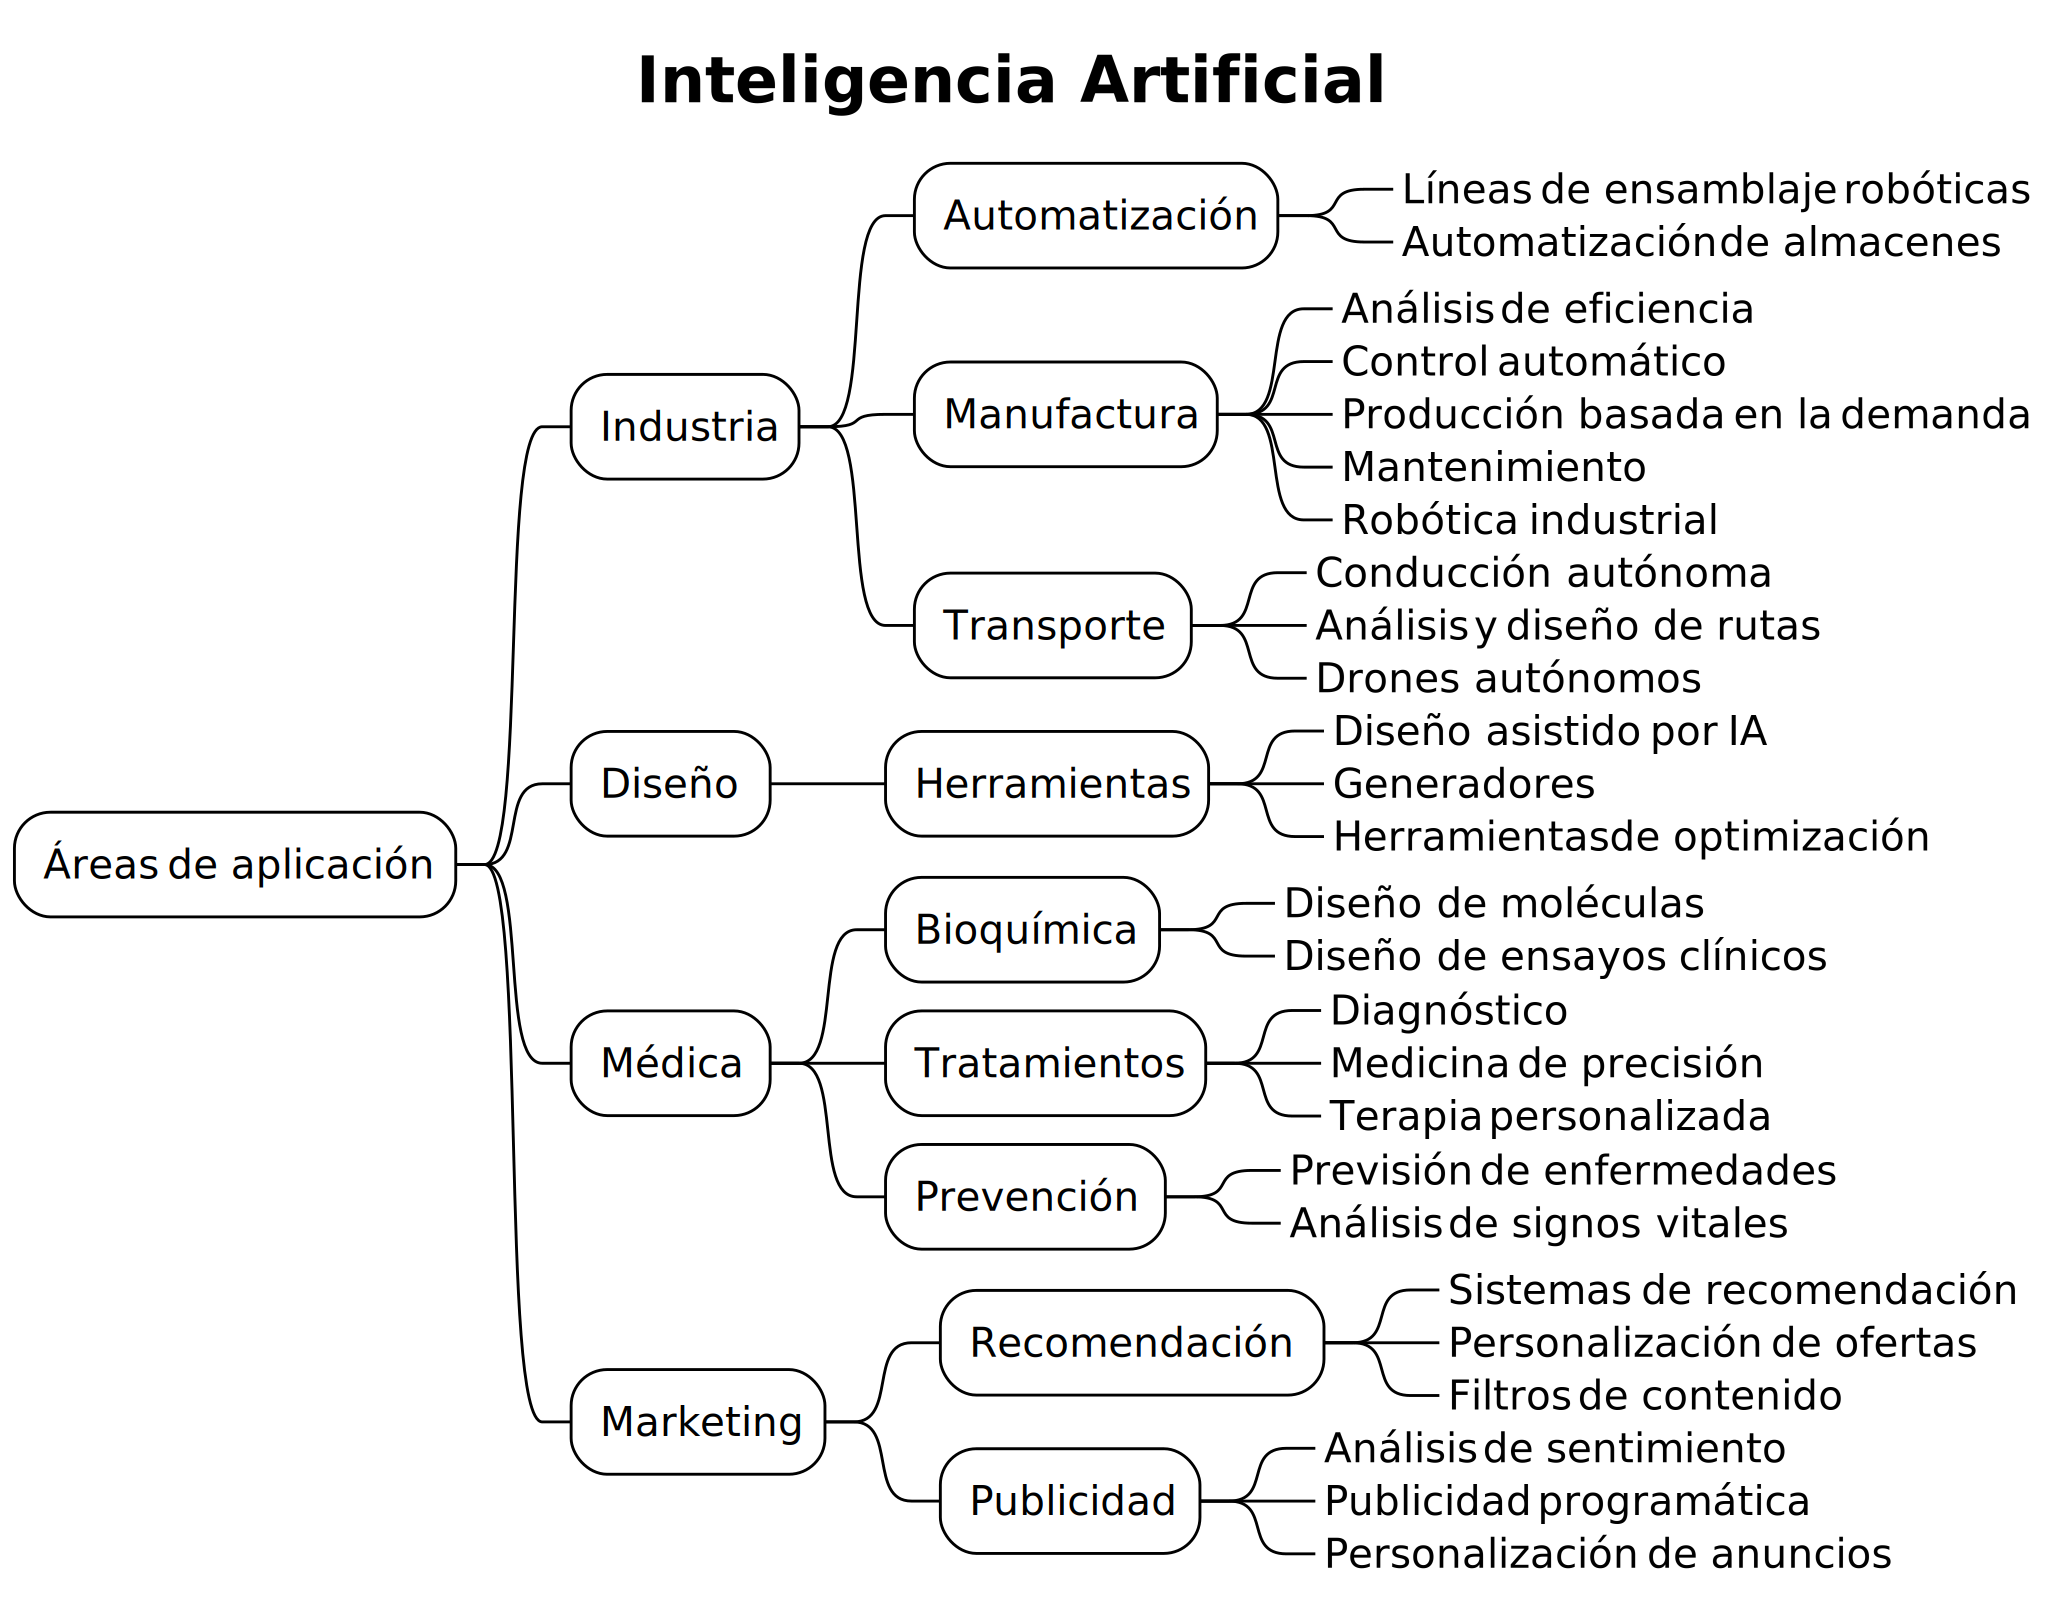
\includegraphics[width=.9\linewidth]{./images/mapa.png}
\end{center}

\pagebreak

\section{Conclusión}
\label{sec:org9131992}
Durante esta practica logre identificar las caracteristicas que hacen a un 
administrador de redesde computadoras ademas de que son las redes de computo, 
como futuros ingenieros en software las redes de computadoras son una herramienta
indispensable debido a la alta interconectividad del mundo actual.

\section{Referencias}
\label{sec:orgb7270c7}
\printbibliography[heading=none]
\end{document}
